\part{Von der visuellen zur textbasierten Programmierung}

\chap{AESL lernen von VPL Programmen}\label{ch.next}

Herzliche Gratulation! Sie sind ein Experte im Programmieren von Thymio mit der \textit{Visuellen Programmierumgebung (VPL)}. Nun wollen Sie weiter gehen zur professionellen \textit{Studio Programmierumgebung} (\cref{fig.studio}) und seiner textbasierten Programmiersprache, der Aseba-Ereignis-Skriptsprache AESL \textit{Aseba Event Scripting Language}.

\begin{figure} 
	\begin{center}
		\gr{studio}{.9}
		\caption{Aseba Studio Programmierumgebung}\label{fig.studio}
	\end{center}
\end{figure}

VPL übersetzt graphische Programme (Ereignis-Aktions-Paare) in ein textbasiertes AESL Programm, welches auf der rechten Seite des VPL-Fensters dargestellt wird (Bereich~6 in der Grafik \cref{fig.vplgui} auf Seite ~\pageref{fig.vplgui}). Im vorliegenden Lernprogramm werden VPL Programme aus den vorherigen Kapiteln verwendet, um die entsprechenden AESL-Programme zu erklären. Sie werden in der Lage sein, Ihre Kenntnis von VPL zu benutzen um die Konzepte von AESL zu erlernen.

Die Programmierung in Aseba Studio basiert wie gehabt auf Ereignissen und Aktionen. Da VPL-Programme in AESL-Programme übersetzt werden, stehen alle VPL-Konstrukte auch in AESL zur Verfügung. Zusätzlich haben Sie die Flexibilität einer normalen Programmiersprache mit Variablen, Ausdrücke und Anweisungen für die Ablaufsteuerung.

Wenn Sie mit Aseba Studio arbeiten, können Sie VPL öffnen, indem Sie den Knopf \bu{Launch VPL} im Bereich \emph{Tools} anwählen (im unteren Bereich des Fensters). Sie können ein VPL-Programm in Aseba Studio importieren, indem Sie einfach das VPL-Dokument öffnen.

Abschnitte die mit $^*$ markiert sind, beschreiben Programmierkonzepte, die über das hinausgehen, was in den VPL-Projekte zu finden ist. Sie können diese Abschnitte überspringen, wenn Sie das Lernprogramm zunächst nur durchlesen wollen. 

\textbf{\large Dokumentation}

Um Aseba Studio und AESL zu lernen, gehen Sie auf die Seite \emph{Programming
Thymio} page at\\
\href{https://www.thymio.org/de:asebausermanual}{https://www.thymio.org/de:asebausermanual}.
Dort finden Sie Unterlagen zu folgenden Themen:

\begin{itemize}
\item Die Programmierumgebung.
\item Die Programmiersprache AESL.
\item Die Schnittstelle des Roboters Thymio.
(Es hat auch eine Referenzkarte zu dieser Schnittstelle).
\item Die Bibliotheksfunktionen, die von AESL unterstützt werden.
\end{itemize}

Des weiteren gibt es eine Sammlung von interessanten AESL-Projekten inkl. Quellcode von vorgeschlagenen Lösungen.

\sect{Die Schnittstelle von Thymio}

Nachfolgend die Darstellung des Programms \p{whistles.aesl} aus \cref{ch.bells} mit einem Ausschnitt aus dem dazugehörenden AESL Programm:
 
\begin{center}
\begin{tabular}{ll}
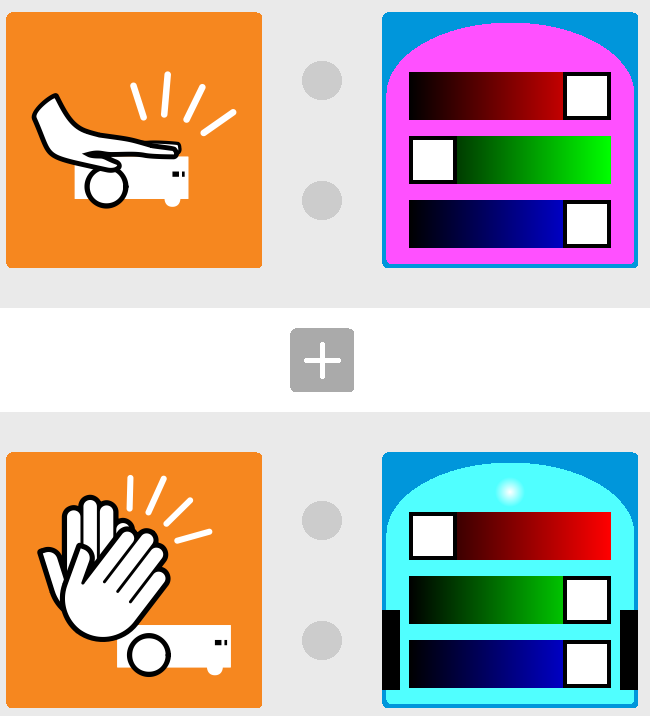
\includegraphics[width=.4\textwidth]{whistles} &
\begin{minipage}[b]{.5\textwidth}
\begin{footnotesize}
\begin{verbatim}
  onevent tap
    call leds.top(32,0,32)
  
  onevent mic
    call leds.bottom.left(0,32,32)
    call leds.bottom.right(0,32,32)
\end{verbatim}
\end{footnotesize}
\vspace*{8ex}
\end{minipage}
\end{tabular}
\end{center}

\textbf{\large Eventhandler (Ereignisbehandlungsroutinen)}

Wenn ein Klopfen-Ereignis eintritt, wird das oberen LED-Licht eingeschaltet in der Farbe \emph{Magenta} (Rotblau, Fuchsia, helles Purpur), und wenn ein Klatschen-Ereignis eintritt werden die unteren Lichter in der Farbe \emph{Cyan} (Blaugrün, Türkis) eingeschaltet. Die Ereignis-Aktions-Paare in VPL sind sogenannte \emph{Eventhandler}, die in AESL durch das Schlüsselwort \p{onevent} eingeführt werden - man liest das englische Schlüsselwort als zwei Wörter ''on event''. Sie finden eine Liste aller Ereignisse in der Programmierumgebung Aseba Studio unten links unter ''Lokale Ereignisse'' aufgelistet (die in den Programmierbereich gezogen werden können).

Die Zeilen, die auf \p{onevent} folgen, bilden den Körper des Eventhandlers und entsprechen den Aktions-Blöcken im rechten Bereich in VPL.

Wenn ein Klopfen-Ereignis eintritt, wird die \emph{Schnittstellen-Funktion} \p{leds.top} aufgerufen. Der Aufruf erfolgt mit drei \emph{Parametern}, welche die Intensität der roten, grünen und blauen Anteile des LED-Lichts angeben. Ihr Wert liegt zwischen 0 (ausgeschaltet) und 32 (voll). Die Mischung aus rot und blau ergibt Magenta (Fuchsia). 

Das Klatschen-Ereignis in VPL entspricht dem  \p{mic} Ereignis in AESL (mic steht als Abkürzung für microphone). Wenn das Ereignis eintritt, werden die unteren LED-Lichter eingeschaltet. In VPL werden beide unteren LED-Lichter mit einem Aktions-Block eingeschaltet. In AESL können die beiden Lichter unterschiedlich und direkt angesteuert werden. Hier werden beide mit voller Stärke auf grün und blau gesetzt, was Cyan (Türkis) ergibt. 

\textbf{\large Einen Wert einer Variablen zuordnen}

Schauen Sie sich das AESL-Programm nochmals an. Die ersten beiden Zeilen lauten wie folgt: 
\begin{footnotesize}
\begin{verbatim}
  # setup threshold for detecting claps
  mic.threshold = 250
\end{verbatim}
\end{footnotesize}

Eine Zeile, die mit einem \verb+#+ beginnt, ist ein \emph{Kommentar}. Kommentare haben keinen Einfluss auf das laufende Programm; sie werden benutzt um dem Leser Informationen weiterzugeben. Der angegebene Kommentar wird vom Übersetzungsprogramm vergeben und bedeutet auf Englisch, dass der Schwellwert für das Klatsch-Ereignis eingestellt werden wird: ein Geräusch, das grösser als \emph{threshold} ist, führt dazu, dass das Ereignis erkannt wird. Die zweite Zeile des Programms spezifiziert nun den Schwellwert mit $250$; ausgelöst wird das Ereignis ab einem Wert von $250$ - der Wertebereich liegt zwischen $0$--$255$.

In VPL ist der Schwellwert fix vorgegeben, wohingegen man im textbasierten Programm den Wert mit einer einfachen \emph{Zuweisung} ändern kann: 
\begin{footnotesize}
\begin{verbatim}
  mic.threshold = 180
\end{verbatim}
\end{footnotesize}
Die Bedeutung der Zuweisung ist, dass der Wert der \emph{Wert} auf der rechten Seite des \verb+=+ (Gleichheitszeichens) in die \emph{Variable} auf der linken Seite kopiert wird. Die Variable \p{mic.threshold} ist vordefiniert (muss daher nicht deklariert werden).

\textbf{\large Initialisierung des Roboters Thymio}

Am Anfang jedes Programms wird eine Reihe von Befehlen eingefügt, die den Sound und alle Lichter aus schalten:

\begin{footnotesize}
\begin{verbatim}
  # reset outputs
  call sound.system(-1)
  call leds.top(0,0,0)
  call leds.bottom.left(0,0,0)
  call leds.bottom.right(0,0,0)
  call leds.circle(0,0,0,0,0,0,0,0)
\end{verbatim}
\end{footnotesize}

Diese \emph{Initialisierung} ist im VPL-Programm nicht zu erkennen. Es wird empfohlen, diese Initialisierung in einem textbasierten Programm zu verwenden, aber dies ist nicht zwingend vorgeschrieben. 

\sect{Fallunterscheidung (Alternativen)}

Das Programm \p{colors-multiple.aesl} aus \cref{ch.colors} wechselt die Farben der oberen und unteren Lichter, wenn die Knöpfe berührt werden:

\begin{center}
\begin{tabular}{ll}
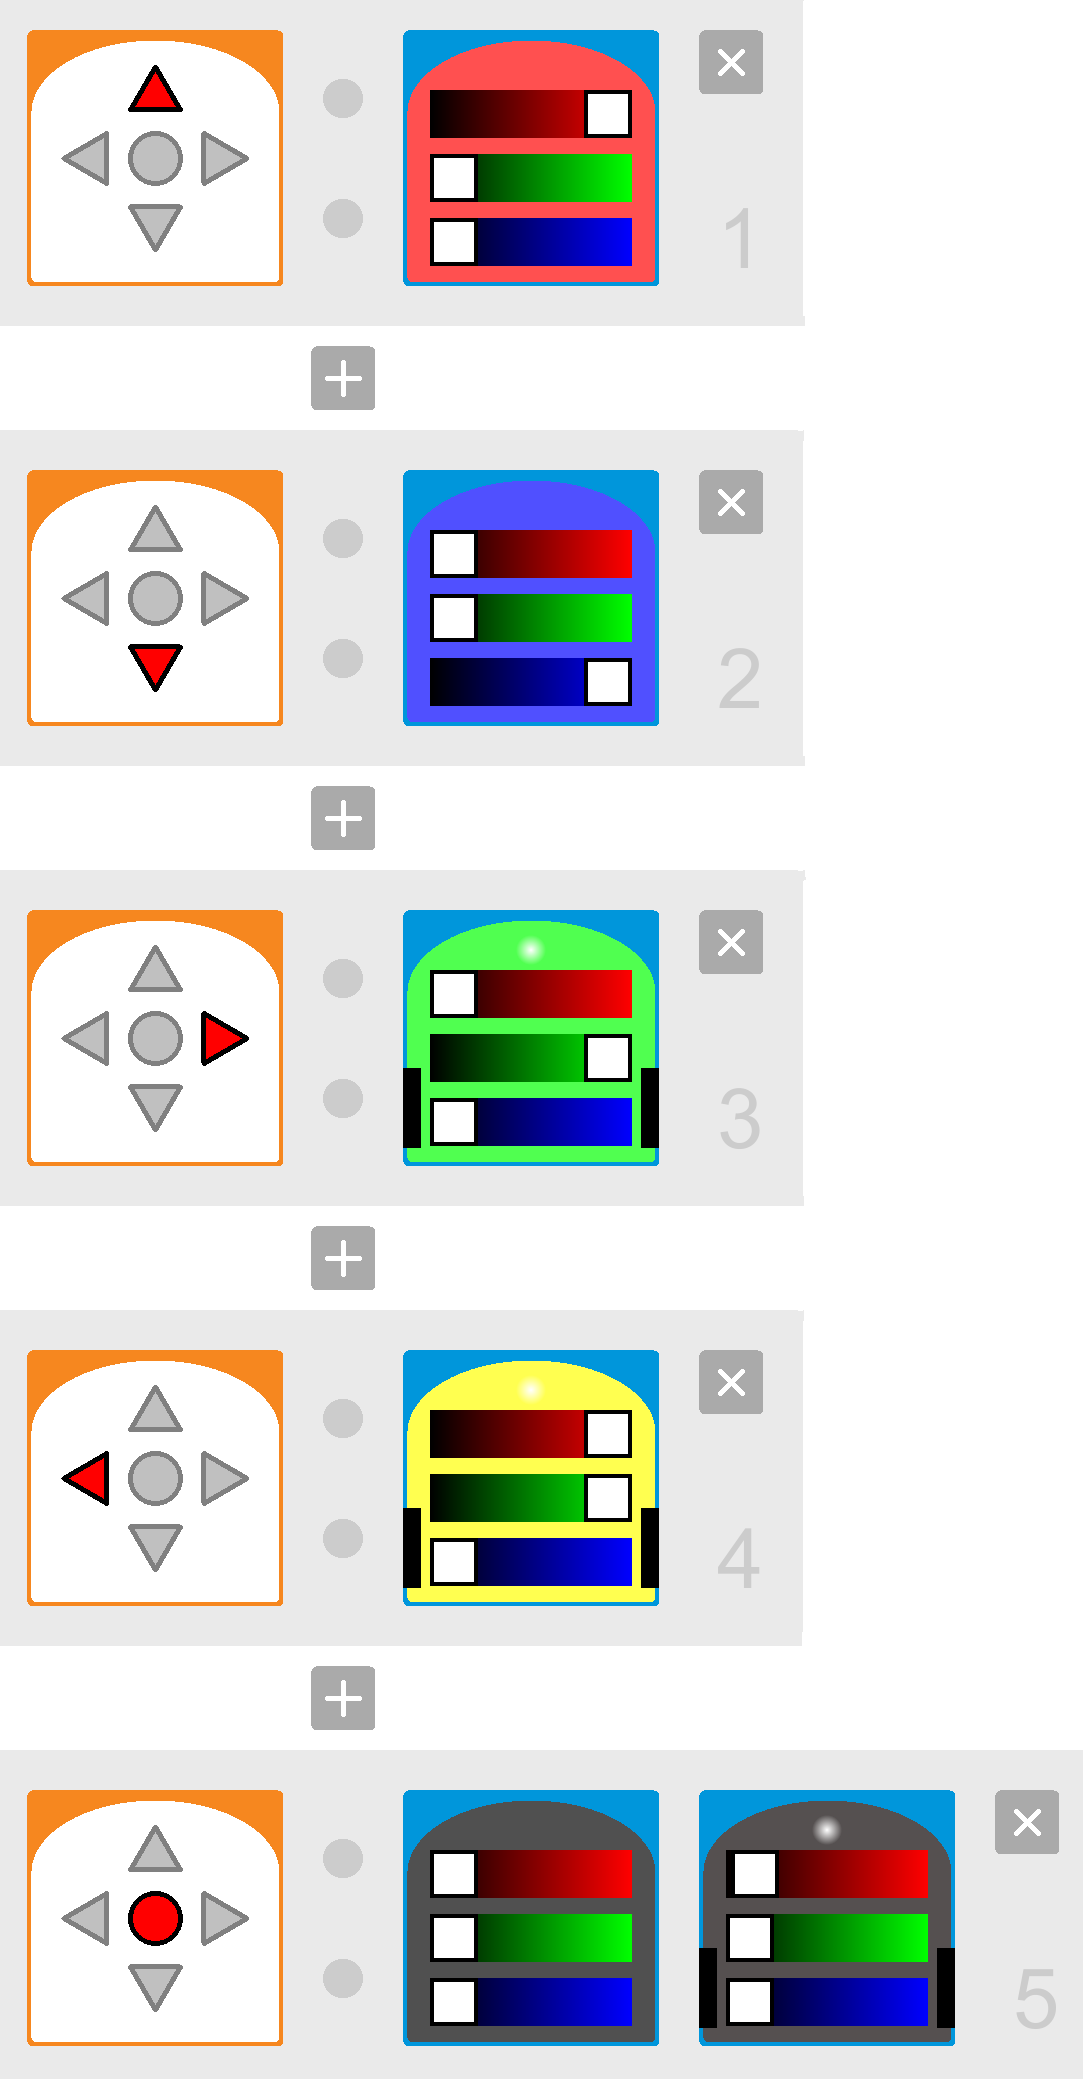
\includegraphics[width=.4\textwidth]{colors-multiple-full} &
\begin{minipage}[b]{.5\textwidth}
\begin{footnotesize}
\begin{verbatim}
  onevent buttons
    when button.forward == 1 do
      call leds.top(32,0,0)
    end
    when button.backward == 1 do
      call leds.top(0,0,32)
    end
    when button.right == 1 do
      call leds.bottom.left(0,32,0)
      call leds.bottom.right(0,32,0)
    end
    when button.left == 1 do
      call leds.bottom.left(32,32,0)
      call leds.bottom.right(32,32,0)
    end
    when button.center == 1 do
      call leds.top(0,0,0)
      call leds.bottom.left(7,0,0)
      call leds.bottom.right(7,0,0)
    end
\end{verbatim}
\end{footnotesize}
\vspace*{5ex}
\end{minipage}
\end{tabular}
\end{center}

Im AESL-Programm tritt ein \emph{einzelnes} Ereignis ein, wenn man einen beliebigen Knopf drückt. Die Aktion des Eventhandlers \p{onevent buttons} hängt davon ab, welcher Knopf gedrückt wurde. Wir müssen daher die \emph{Variable} \p{button} untersuchen, um die richtige Aktion auswählen zu können:

\begin{footnotesize}
\begin{verbatim}
  when button.forward == 1 do
    call leds.top(32,0,0)
  end
\end{verbatim}
\end{footnotesize}

bedeutet \emph{when} (falls) der Wert der Variablen \p{button.forward} von einem Wert (hier: 0) auf 1 ändert, \emph{dann} wird die beschriebene Aktion ausgeführt, die sich zwischen den Schlüsselwörtern \p{do} und \p{end} befindet bzw. befinden.
Es gibt fünf \p{button}-Variablen, eine für jeden Knopf. Der Wert der Variablen ist 1, wenn der Knopf gedrückt wurde und 0 wenn der Knopf losgelassen wurde. Eine oder zwei Aktionen werden ausgeführt, wenn ein \p{when}-Fall wahr \emph{wird}.

\textbf{\large Ein Ereignis oder mehrere Ereignisse$^*$}

Die Schnittstelle von Thymio umfasst eigene Ereignisse für jeden Knopf sowie zusätzlich das oben beschriebene \p{buttons} Ereignis, welches zutrifft, wenn irgend ein Knopf gedrückt oder losgelassen wurde. Wir könnten das Programm daher auch folgendermassen implementieren, unter Verwendung von mehreren Ereignissen und ohne die \p{when}-Anweisung und button-Variablen:

\begin{footnotesize}
\begin{verbatim}
  onevent button.forward
    call leds.top(32,0,0)
  
  onevent button.backward
    call leds.top(0,0,32)
  
  onevent button.right
    call leds.bottom.left(0,32,0)
    call leds.bottom.right(0,32,0)
  
  onevent button.left
    call leds.bottom.left(32,32,0)
    call leds.bottom.right(32,32,0)
  
  onevent button.center
    call leds.top(0,0,0)
    call leds.bottom.left(1,0,0)
    call leds.bottom.right(1,0,0)
\end{verbatim}
\end{footnotesize}

Der Vorteil bei der Verwendung von mehreren Ereignissen ist, dass das Programm leichter lesbar ist, aber es gibt Fälle, wo man das Ereignis \p{buttons} nehmen muss:  (a) um zu unterscheiden, ob der Knopf gedrückt oder losgelassen wird,
und (b) um festzustellen, dass zwei Knöpfe gleichzeitig gedrückt wurden:

\begin{footnotesize}
\begin{verbatim}
  onevent buttons
    # Turn the top LEDs on when the forward button is released
    when button.forward == 0 do
      call leds.top(32,0,0)
    end

    # Turn the bottom LEDs on when
    #   both the left and the right buttons are  touched
    when button.left == 1 and button.right == 1 do
      call leds.bottom.left(0,32,0)
      call leds.bottom.right(0,32,0)
    end
\end{verbatim}
\end{footnotesize}

Ein weiterer Unterschied ist, dass die individuellen Ereignisse immer eintreten, wenn ein Knopf gedrückt oder losgelassen wird, wohingegen das einfache Ereignis \p{buttons} in regelmässigen Abständen untersucht wird (mit einer Frequenz von 20 Hz; mehr zu diesem Konzept auf Seite~\pageref{pg.hz}).
\newpage
\textbf{\large \p{if}- und \p{when}-Anweisung\label{p.if-when}}

AESL unterstützt zwei alternative Anweisungen:
\begin{footnotesize}
\begin{verbatim}
  when v == 1 do ... statements ... end

  if v == 1 then ... statements ... end
\end{verbatim}
\end{footnotesize}
deren Bedeutung sich wie folgt unterscheidet: 
\begin{quote}
\emph{when} der Wert von \p{v} 1 \emph{wird}, führe die Befehle aus

\emph{if} der Wert von \p{v} 1 \emph{ist}, führe die Befehle aus
\end{quote}

\p{when}-Anweisungen werden üblicherweise verwendet bei Variablen, die ein Ereignis darstellen, denn üblicherweise wollen wir Befehle ausführen, wenn etwas ändert und nicht wenn eine Variable einen bestimmten Wert hat. Wir könnten ein \p{buttons}-Ereignis mit einem Eventhandler implementieren, der \p{if}-Anweisungen verwendet:

\begin{footnotesize}
\begin{verbatim}
  onevent buttons
    if button.forward == 1 then
      ... statements ...
    end
\end{verbatim}
\end{footnotesize}
Allerdings werden in diesem Fall die Befehle mehrfach ausgeführt, wenn wir längere Zeit auf den Knopf drücken. Wenn die Befehle nur dir Farbe ändern, macht es zwar keinen grossen Unterschied, aber es gibt Fälle, wo es einen Unterschied macht und man eine \p{when}-Anweisung nehmen muss.

Eine \p{if}-Anweisung ist geeignet, wenn uns der Wert einer Variable interessiert und nicht ihre Änderung. Die Nachfolgenden Befehle setzen den Wert der Variable \p{max} auf das Maximum der erhaltenen beiden Sensorwerte der unteren Distanz-Sensoren: 

\begin{footnotesize}
\begin{verbatim}
  if prox.horizontal[5] > prox.horizontal[6] then
    max = prox.horizontal[5]
  else
    max = prox.horizontal[6]
  end
\end{verbatim}
\end{footnotesize}

Weitere Beispiele für die \p{if}-Anweisung finden sich im nächsten Abschnitt und in der Abbildung~\ref{fig.respond}.


\newpage

\sect{Arrays (Felder)}

Das Programm \p{likes.aesl} im \cref{ch.pet} programmiert den Roboter so, dass er Ihrer Hand folgt, wenn man sie vor den horizontalen Distanzsensoren hin und her bewegt. Wenn kein Objekt erkannt wird, hält der Roboter an; wenn ein Objekt vom mittleren Sensor erkannt wird, fährt der Roboter vorwärts; wenn ein Objekt von der äusseren Sensoren links oder rechts erkannt wird, dann dreht er sich in die jeweilige Richtung. 

\begin{figure}[hbt]
\begin{center}
\begin{tabular}{lr}
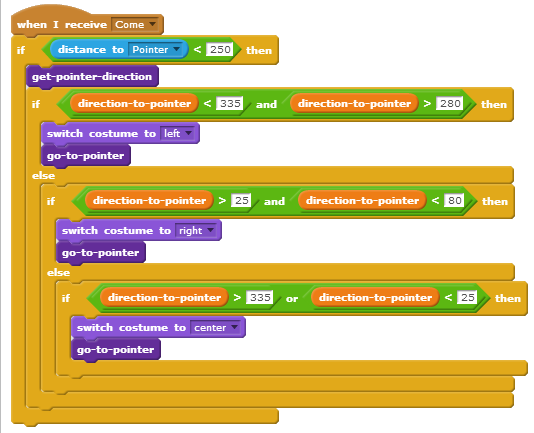
\includegraphics[width=.35\textwidth]{likes} &
\begin{minipage}[b]{.4\textwidth}
\begin{footnotesize}
\begin{verbatim}
  onevent prox
    when prox.horizontal[2] < 1000 do
      motor.left.target = 0
      motor.right.target = 0
    end
    when prox.horizontal[2] > 2000 do
      motor.left.target = 300
      motor.right.target = 300
    end
    when prox.horizontal[0] > 2000 do
      motor.left.target = -300
      motor.right.target = 300
    end
    when prox.horizontal[4] > 2000 do
      motor.left.target = 300
      motor.right.target = -300
    end
\end{verbatim}
\end{footnotesize}
\end{minipage}
\end{tabular}
\caption{Das Programm''\p{likes}'' in VPL und AESL}\label{fig.arrays}
\end{center}
\end{figure}

Das AESL-Programm (\cref{fig.arrays}) besteht aus einem Eventhandler mit mehreren \p{when}-Anweisungen. Die Werte der Motoren-Variablen \p{motor.left.target} und \p{motor.right.target} wurden auf Werte gesetzt, die der Position der Schieberegler im Motoren-Block entspricht. In VPL ändern die Werte in $50$er-Schritten, aber in AESL kann man sie auf einen beliebigen Wert zwischen $-500$ und $500$ setzen.

Das Ereignis wird \p{prox} genannt (kurz für proximity = Nähe). Im Gegensatz zu den Knopf-Ereignissen, welche eintreten, wenn etwas ''pasiert'', tritt dieses Ereignis \emph{10 Mal pro Sekunde} ein. Bevor das Ereignis eintritt, werden die von den Sensoren gemessenen Werte in die Variable \p{prox.horizontal} gespeichert. Details hierzu finden sich in der \label{pg.hz} Dokumentation zur Thymio-Programmierschnittstelle. \footnote{Die Einheit für die \emph{Frequenz}, also die Angabe, wie oft etwas pro Sekunde passiert, nennt man \emph{Hertz}, abgekürzt \emph{Hz}. Das Dokument zur Schnittstelle spezifiziert, dass das {\footnotesize\p{prox}}-Ereignis mit einer Frequenz von \emph{10 Hz} eintritt, also alle 100ms.}

\textbf{\large Multiple Variablen in einem Array}

Der Roboter Thymio besitzt 7 horizontale Distanz-Sensoren, 5 vorne und 2 hinten. Um die Werte zu lesen, die dieses Sensoren messen, könnte man 7 verschiedene Variablen definieren: 

\begin{footnotesize}
\begin{verbatim}
  prox.horizontal.front.0
  prox.horizontal.front.1
  prox.horizontal.front.2
  prox.horizontal.front.3
  prox.horizontal.front.4
  prox.horizontal.back.0
  prox.horizontal.back.1
\end{verbatim}
\end{footnotesize}

In AESL kann man stattdessen ein \emph{array} definieren, welches eine Abfolge von Variablen darstellt, die alle denselben Namen haben. Die unterschiedlichen Variablen im Array werden durch eine Zahl identifiziert. Das Array für die horizontale Distanz-Sensoren ist vordefiniert und heisst \p{prox.horizontal}:

\begin{center}
\begin{picture}(240,40)
\put(0,0){\makebox(100,20)[l]{\p{prox.horizontal}}}
\put(100,0){\framebox(140,20){}}
\multiput(120,0)(20,0){6}{\line(0,1){20}}
\put(100,20){\makebox(20,20){\p{0}}}
\put(120,20){\makebox(20,20){\p{1}}}
\put(140,20){\makebox(20,20){\p{2}}}
\put(160,20){\makebox(20,20){\p{3}}}
\put(180,20){\makebox(20,20){\p{4}}}
\put(200,20){\makebox(20,20){\p{5}}}
\put(220,20){\makebox(20,20){\p{6}}}
\end{picture}
\end{center}

Die ersten 5 Elemente sind für die vorderen Sensoren von links bis recht und die letzten beiden Elemente für die hinteren beiden Sensoren wieder von links nach rechts. Sollten Sie diese Zuordnung vergessen, schauen Sie in der Dokumentation nach oder noch besser auf der Referenzkarte. 

Um auf eine Variable in einem Array zugreifen zu können, schreibt man seine Zahl in eckigen Klammern nach dem Variablennamen. Diese Zahl nennt man \emph{Index} des Arrays. Die nachfolgende Befehlsfolge legt fest, dass die Motoren-Variablen auf 300 festgelegt werden, wenn der \emph{mittlere Distanzsensor} (index 2) grösser als 2000 wird:

\begin{footnotesize}
\begin{verbatim}
  when prox.horizontal[2] > 2000 do
    motor.left.target = 300
    motor.right.target = 300
  end
\end{verbatim}
\end{footnotesize}

Später werden wir sehen, dass Array-Variablen mit einer Zuweisung der folgenden Art festgelegt werden können: 
\begin{footnotesize}
\begin{verbatim}
  timer.period[0] = 1979
\end{verbatim}
\end{footnotesize}

\textbf{\large \p{for}-Schleifen und Index-Variablen$^*$}

Man Verallgemeinert die Verwendung eines Arrays, indem man eine Variable für den Index verwendet, anstelle einer Konstante. \footnote{Bei der Übersetzung des Programms aus VPL in AESL wird dies nicht gemacht, ausser bei einem fortgeschrittenen Konstrukt für Töne; daher wird hier das einfache Beispiel aus dem AESL-Projekt genommen.} Das Programm \p{cats.aesl} enthält folgende Befehle: 

\begin{footnotesize}
\begin{verbatim}
  var i

  for i in 0:4 do
    if prox.horizontal[i] > DETECTION then
      state = 2
    end
  end
\end{verbatim}
\end{footnotesize}

Bisher hatten wir nur Variablen benutzt, die bereits in der Schnittstelle von Thymio eingabaut waren; hier nun \emph{deklariert} die erste Zeile eine neue Variable mit Namen \p{i}. Die nächste Anweisung ist eine \p{for}-Anweisung mit folgender Bedeutung: 

\begin{itemize}
\item weise den Wert 0, 1, 2, 3, 4 nachfolgend der Variable \p{i} zu;
\item für jede Zuweisung führe die Befehle zwischen \p{do} und \p{end} aus.
\end{itemize}

Im vorliegenden Fall gibt es nur eine einzelne \p{if}-Anweisung zwischen \p{do} und \p{end}. Dabei wird der Wert der horizontalen Distanzsensoren untersucht und der Wert der Variable \p{state} wird auf 2 gesetzt, falls der gemessene Wert grösser ist als die Konstante \p{DETECTION}.\footnote{Hinweise zur Definition von Konstanten finden Sie in der Aseba-Studio Dokumentation.}

Die Variable \p{i} bekommt nacheinander die Werte 0, 1, 2, 3 und 4, daher wird jedes Mal, wenn die \p{if}-Anweisung ausgeführt wird mit \p{prox.horizontal[i]} ein anderer Sensor untersucht. Das Ergebnis der \p{for}-Anweisung ist daher dass die Variable \p{state} auf 2 gesetzt wird, \emph{falls} \emph{irgendeiner} der vorderen Distanzsensoren ein Objekt erkennt.

\textbf{\large Deklarieren eines Arrays}

Ein Array wird deklariert, indem man seinen Namen angibt gefolgt von seine Grösse in eckigen Klammern. Bei der Deklaration kann man auch den Wert der Komponenten (Variablen an den einzelnen Indexpositionen) angeben:\footnote{Ein Kommentar muss nicht am Anfang einer Zeile stehen. Jedes Zeichen zwischen dem Zeichen \# und dem Ende der Zeile wird durch den Computer ignoriert.}

\begin{footnotesize}
\begin{verbatim}
var state[4]             # Ein Array mit vier Komponenten  
var state[] = [0,0,0,0]  # Ein Array mit vier Komponenten vom Wert 0
\end{verbatim}
\end{footnotesize}

In der Übersetzung des VPL-Programms werden Grösse und initialer Wert der Komponenten festgelegt. Dies funktioniert, so lange die Grösse und die Anzahl Werte übereinstimmen:

\begin{footnotesize}
\begin{verbatim}
var state[4] = [0,0,0,0]  # OK, aber redundant
\end{verbatim}
\end{footnotesize}

\newpage

\sect{Timer}

In \cref{ch.time} wurden \emph{Timer} eingeführt. Das Programm \p{shy.aesl} bringt den Roboter nach links auszuweichen, wenn der mittlere vordere Sensor Ihre Hand entdeckt; zwei Sekunden später weicht er nach rechts aus: 

\begin{center}
\begin{tabular}{ll}
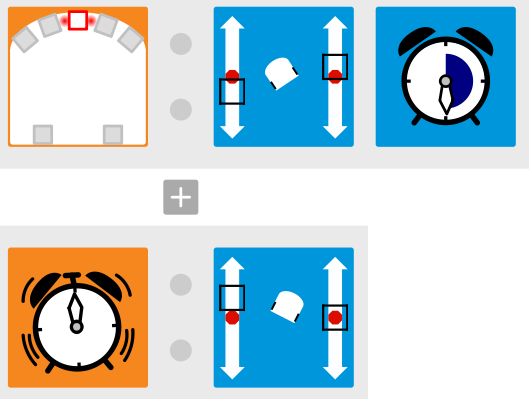
\includegraphics[width=.4\textwidth]{shy} &
\begin{minipage}[b]{.5\textwidth}
\begin{footnotesize}
\begin{verbatim}
  onevent prox
    when prox.horizontal[2] > 2000 do
      motor.left.target = -150
      motor.right.target = 100
      timer.period[0] = 2000
    end
  
  onevent timer0
    timer.period[0] = 0
    motor.left.target = 200
    motor.right.target = 0
\end{verbatim}
\end{footnotesize}
%\vspace*{1ex}
\end{minipage}
\end{tabular}
\end{center}

Im Roboter Thymio gibt es zwei Timer. Sie werden den beiden Werten des Arrays \p{timer.period} zugewiesen. Wenn Sie eine Dauer zuweisen, verwenden Sie entweder die Komponente 0 oder 1 aus dem Array. Der Wert der Dauer wird in \emph{Millisekunden} angegeben, also in Tausendsteln einer Sekunde. Wenn wir eine Dauer von 2 Sekunden im Timer 0 festlegen wollen, schreiben wir daher \p{timer.period[0] = 2000}.

Es gibt 2 Ereignisse, \p{timer0} und \p{timer1}, ein Ereignis für beide Timer. Wenn die Zeit vorbei ist, d.h. wenn der Timer \emph{abgelaufen} ist, tritt das Ereignis ein. Im Eventhandler für das Ereignis \p{timer0} legen wir die Dauer mit 0 fest, damit das Ereignis nicht nochmal eintritt und die Einstellungen des Motors verändert.

Bei der Initialisierung des Timers wird der Timerwert auf 0 gesetzt, damit die Aktion nicht aus Versehen startet:

\begin{footnotesize}
\begin{verbatim}
  # stop timer 0
  timer.period[0] = 0
\end{verbatim}
\end{footnotesize}

\sect{Zustände}

In \cref{ch.states,ch.counting} wurde die Verwendung von \emph{Zuständen} erklärt. Der Roboter Thymio kann sich in einem von 16 Zuständen befinden und man kann spezifizieren, dass ein Ereignis nur dann eine Aktion auslöst, wenn sich der Roboter in einem bestimmten Zustand befindet. Im Programm \p{count-to-two.aesl} aus \cref{ch.counting} wird der Zustand auf 0 gesetzt, wenn der mittlere Knopf gedrückt wurde; danach zählt er die Anzahl Geräusche (Klatschen) und gibt en, ob es eine gerade oder ungerade Anzahl ist, indem abwechselnd der Zustand auf 0 und 1 gesetzt wird. Das VPL Programm und seine AESL-Übersetzung für die Berührung des mittleren Knopfes sind:\footnote{Das hier abgebildete AESL-Programm unterscheidet sich vom generierten Programm, was später in diesem Kapitel erklärt wird.}

\begin{center}
\begin{tabular}{ll}
\raisebox{8ex}{
\includegraphics[width=.4\textwidth]{two-button}} &
\begin{minipage}[b]{.5\textwidth}
\begin{footnotesize}
\begin{verbatim}
  var state[] = [0,0,0,0]
  
  onevent buttons
    when button.center == 1 do
      state[0] = 0
      state[1] = 0
      state[2] = 0
      state[3] = 0
    end
\end{verbatim}
\end{footnotesize}
\end{minipage}
\end{tabular}
\end{center}

Der Zustand wird in einem Array \p{state[]} gespeichert, der 4 Komponenten besitzt. Jede Komponente kann den Wert 0 oder 1 haben, daher gibt es $2\times 2\times 2\times 2=16$ mögliche Werte für die Werte des Arrays. Den Komponenten des Arrays werden bei der Initialisierung allen der Wert 0 zugewiesen: {\footnotesize\verb+[0,0,0,0]+}. Mit der Initialisierung wird gleichzeitig die Grösse des Arrays festgelegt; da es hier 4 Werte sind in {\footnotesize\verb+[0,0,0,0]+}, gibt es auch 4 Komponenten im Array.

Der Ereignis-Zustandsblock (grün, neben dem Knopf-Ereignisblock) ist dunkelgrau in allen 4 Vierteln; das bedeutet, dass das Ereignis eintreten kann, unabhängig vom Wert der Zustandsvariablen. Daher wird, wenn der mittlere Knopf betätigt wird, die Status-Aktion ausgeführt (blau) was dazu führt, dass alle Komponenten des Arrays \p{state} auf 0 gesetzt werden, was durch die weissen Viertel angezeigt wird. 

Im entsprechenden AESL-Programm untersucht die \p{when}-Anweisung ob der mittlere Knopf gedrückt wurde, aber nicht, welche Werte die Komponenten des Arrays \p{state} hatten. Wenn der Knopf gedrückt wird, werden alle Komponenten auf 0 gesetzt. 

Es gibt zwei Klatsch-Ereignis-Blöcke, jeder verbunden mit einem anderen Zustands-Block.
Im textbasierten Programm wird ein einzelnen Eventhandler \p{mic} verwendet. Die Anweisungen, die im jeweiligen Fall zu befolgen sind, hängen von den abgefragten Werten in der \p{if}-Anweisung ab (\cref{fig.respond}).

\begin{figure}[hbt]
\begin{center}
\begin{tabular}{ll}
\raisebox{10ex}{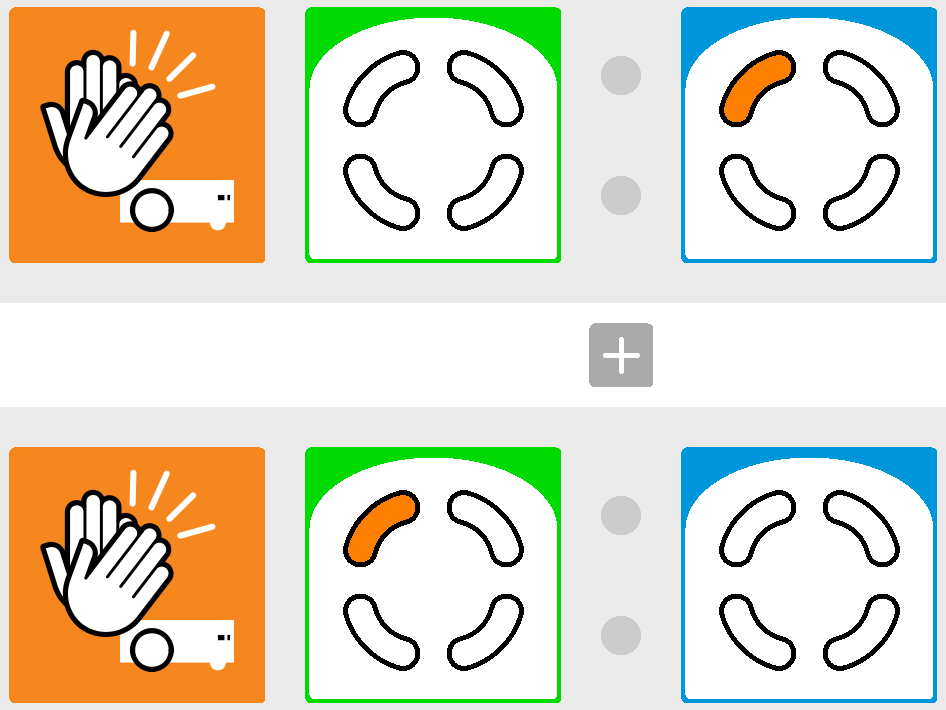
\includegraphics[width=.4\textwidth]{two-clap}} &
\begin{minipage}[b]{.5\textwidth}
\begin{footnotesize}
\begin{verbatim}
  onevent mic
    if state[0] == 0 and
       state[1] == 0 and
       state[2] == 0 and
       state[3] == 0 then
      state[0] = 1
      state[1] = 0
      state[2] = 0
      state[3] = 0
    end
    if state[0] == 1 and
       state[1] == 0 and
       state[2] == 0 and
       state[3] == 0 then
      state[0] = 0
      state[1] = 0
      state[2] = 0
      state[3] = 0
    end
\end{verbatim}
\end{footnotesize}
\end{minipage}
\end{tabular}
\caption{Reaktion auf Klatschen abhängig vom Zustand}\label{fig.respond}
\end{center}
\end{figure}

Die Bedeutung des Schlüsselwortes \p{and} ist, dass \emph{alle} Bedingungen in der \p{if}-Anweisung erfüllt sein müssen, damit die Befehle zwischen \p{then} und \p{end} ausgeführt werden. Wenn alle Komponenten von \p{state} den Wert 0 haben, wird der Wert der Komponente \p{state[0]} auf 1 gesetzt, und die anderen werden auf 0 gesetzt. Dies entspricht dem Zustands-Ereignis-Block mit allen Vierteln auf weiss eingestellt und dem Aktions-Ereignis-Block mit dem Viertel oben links auf orange\footnote{Man könnte sich auf die Behandlung des ersten Viertels beschränken oder die Zustandswerte, die nicht geändert werden sollen, so belassen, wie sie sind, doch hilft es, Fehler zu vermeiden, wenn man die Werte explizit angibt und ändert.}. 
In gleicher weise wird der Wert von \p{state[0]} untersucht: ist er 1 und alle anderen Komponenten 0, dann werden alle Komponenten auf 0 gesetzt. 

\sect{Unterprogramme}

Es kommt relativ häufig vor, dass man dieselbe Sequenz von Anweisungen an vielen Stellen im Programm wieder verwenden muss. Wir können diese Anweisungen ein Mal schreiben und dann x Mal kopieren. Eine einfachere Lösung ist, ein \emph{Unterprogramm} zu verwenden, welches aus einem Namen und einer Sequenz von Anweisungen besteht. In diesem Programm wird die Deklaration {\footnotesize\verb+sub display_state+} verwendet, um dem Unterprogramm {\footnotesize\verb+display_state+} eine Sequenz von Befehlen zuzuweisen (hier bestehend aus einem einzigen Befehl auf zwei Zeilen: \p{call leds.circle}):

\begin{footnotesize}
\begin{verbatim}
  # Unterprogramm zur Darstellung des aktuellen Zustands
  sub display_state
    call leds.circle(
      0, state[1]*32, 0, state[3]*32, 0, state[2]*32, 0, state[0]*32)
\end{verbatim}
\end{footnotesize}

Wenn das Unterprogramm \emph{aufgerufen} wird, ruft es seinerseits die Anweisungen auf, die bei der Definition des Unterprogramms angegeben wurden: 
\vspace{-1ex}
\begin{footnotesize}
\begin{verbatim}
  callsub display_state
\end{verbatim}
\end{footnotesize}
\vspace{-1ex}
Die Schnittstellen-Funktion \p{leds.circle} legt die Lichtstärke der abgerundeten acht LED-Lichter fest, die um die Knöpfe herum angebracht sind. Sie müssen die Referenzkarte konsultieren um zu sehen, welcher Parameter welches LED-Licht festlegt!

Die Intensität der einzelnen LED-Lichter wird festgelegt, indem man dem entsprechenden Parameter einen Wert zwischen 0 (ausgeschaltet) und 32 (voll eingeschaltet) zuweist. Das vordere, rechte, hintere und linke LED-Licht wird ausgeschaltet, indem man ihnen den Wert 0 zuweist; den diagonal angeordneten LED-Lichtern wird der Wert des entsprechenden Zustands-Viertels zugewiesen. Dies geschieht, indem man den \emph{arithmetischen Ausdruck} \p{state[...]*32} verwendet, der den Wert der Komponente im Array mit 32 multipliziert. Wenn der Wert der Zustands-Komponente 0 ist, wird der Parameter 0 übergeben, wenn er 1 ist, wird 32 übergeben. 

\newpage

\sect{Eingebaute (mitgelieferte) Funktionen (native functions)}

Das obige Programm hat ein Problem. Da den Komponenten des Arrays \p{state} einer nach dem anderen Werte zugewiesen werden, ist es möglich dass ein anderes Ereignis eintritt wenn einigen aber noch nicht allen Komponenten des Arrays Werte zugewiesen wurden. Um dies zu verhindern und alle Komponenten eines Arrays gleichzeitig Werte zuzuweisen, werden die Werte zunächst einem zweiten Array (\p{new\_state}) zugewiesen und dann wird der zweite in den ersten (\p{state}) Array kopiert:

\begin{footnotesize}
\begin{verbatim}
# variables for state
var state[4] = [0,0,0,0]
var new_state[4] = [0,0,0,0]

onevent buttons
  when button.center == 1 do
    new_state[0] = 0
    new_state[1] = 0
    new_state[2] = 0
    new_state[3] = 0
  end

  call math.copy(state, new_state)
  callsub display_state
\end{verbatim}
\end{footnotesize}

Die \emph{eingebaute Funktion} \p{math.copy} wird verwendet um Arrays zu kopieren. Eingebaute oder mitgelieferte Funktionen sind in den Roboter Thymio eingebaut und sind effizienter als Sequenzen von Anweisungen in AESL. Die eingebauten Funktionen sind in der Aseba-Dokumentation beschrieben. 

Die aktuelle Version von AESL erlaubt die Zuweisung eines Arrays an einen anderen Array, es wäre also möglich die folgende Zuweisung zu verwenden:\footnote{Die Zuweisung eines Arrays an einen anderen Array wird in eine Sequenz von Zuweisungen für jede Komponente übersetzt, so dass dies unser Problem nicht lösen würde.}

\begin{footnotesize}
\begin{verbatim}
  state = new_state
\end{verbatim}
\end{footnotesize}
